\section{Application 1: Whitened Variational Gaussian Processes}
\label{sec:variational_results}

As a first application of the CIQ method, we will demonstrate that the scalable whitening procedure $\bK^{-1/2} \bb$ can accelerate and increase the fidelity of variational Gaussian process approximations \cite{hensman2013gaussian,hensman2015scalable,matthews2017scalable}.
The whitening operation is commonly used with variational approximations to accelerate the learning of variational parameters \cite{matthews2017gpflow}.


\paragraph{Whitened Stochastic Variational Gaussian Processes.}
Stochastic variational Gaussian processes (SVGP) are used when the data are modelled with non-conjugate likelihoods (e.g. classification) or for large datasets that might not fit into memory.
Recall from \cref{sec:variational} that these models form an approximate predictive distribution
\[
  p(f(\bx) \mid \bX, \by) \approx \Evover{q(\bu)}{ p\left( f(\bx) \mid \bu \right)} = \normaldist{ \bxtest; \ameantest{ \bx }} { \avartest{ \bx }},
\]
where $q \left( \bu \right)$ is a Gaussian distribution parameterized by mean $\bm \in \reals^M$ and covariance $\bS \in \reals^{M \times M}$.
$\bm$ and $\bS$ (as well as inducing point locations $\bZ$ and kernel/likelihood hyperparameters) are chosen to optimizing the variational ELBO (\cref{eqn:elbo}):
%
\begin{align*}
	-\loglik_\text{ELBO} &= -\sum_{i=1}^N \Evover{q(f(\bx^{(i)}))}{  \: \log p( y^{(i)} \mid f(\bx^{(i)}) ) \: } + \kl{ q(\bu) }{ p(\bu) }.
\end{align*}
%
As stated in \cref{sec:variational}, the ELBO factorizes over all data points in the training set $\bX, \by$.
Therefore, it can be approximated using minibatches and used in conjunction with stochastic gradient optimization.

Rather than directly learning $\bm$ and $\bS$, it is more common to learn the \emph{whitened parameters} \cite{kuss2005assessing,matthews2017scalable}:
\[ \bm' = \bK_{\bZ\bZ}^{-\frac 1 2} \bm, \quad \bS' = \bK_{\bZ\bZ}^{-\frac 1 2} \bS \bK_{\bZ\bZ}^{-\frac 1 2} \]
Under this coordinate system, the KL divergence term is given by
%
\begin{equation}
	\kl{ q(\bu') }{ p(\bu') } = \frac{1}{2} \Bigl( \bm^{\prime \top} \bm' + \tr{ \bS' } - \log \vert \bS' \vert - M \Bigr),
	\label{eqn:kldiv_whitened}
\end{equation}
%
which, importantly, doesn't depend on $k(\cdot,\cdot)$ or $\bZ$ and therefore is relatively simple to optimize.
With whitening, the predictive mean and variance of become:
%
\begin{align}
  \ameantest{\bx} &= \bk_{\bZ\bx}^\top \bK_{\bZ\bZ}^{-\frac 1 2} \bm'
  \label{eqn:approx_pred_mean} \\
  \avartest{\bx} &= k(\bx, \bx) -
    \bk_{\bZ\bx}^\top \bK_{\bZ\bZ}^{-\frac 1 2} \left( \bI - \bS' \right) \bK_{\bZ\bZ}^{-\frac 1 2} \bk_{\bZ\bx}
  \label{eqn:approx_pred_covar}
\end{align}
%
During training, we repeatedly compute the ELBO and its derivative, which requires computing \cref{eqn:approx_pred_mean,eqn:approx_pred_covar} for a minibatch of data points.
Optimization typically requires up to $10,\!000$ iterations of training \citep[e.g.][]{salimbeni2018natural};
therefore, we must compute $\bK_{\bZ\bZ}^{- \frac 1 2} \bk_{\bZ \bx_i}$ and its derivative \emph{thousands of times} over the course of training.

\paragraph{Time and space complexity.}
We note that $\bK_{\bZ\bZ}^{-\frac 1 2} \bb$ is the most expensive numerical operation when computing the ELBO and its derivative.
Therefore, the complexity of Cholesky-based SVGP is $\bigo{M^3}$ (the cost of Cholesky-decomposing $\bK_{\bZ\bZ}$).
On the other hand, CIQ-based SVGP is $\bigo{J M^2}$, where $J$ is the number of msMINRES iterations.
Both methods require $\bigo{M^2}$ storage for the $\bm'$ and $\bS'$ parameters.

\subsection{Natural gradient descent with CIQ}
As $M$ increases, the size of the variational parameters $\bm'$ and $\bS'$ grows quadratically.
This poses a more challenging optimization problem for standard gradient descent methods.
To adapt to this parameter increase, we rely on {\bf natural gradient descent (NGD)} to optimize the $\bm'$ and $\bS'$ parameters \citep[e.g.][]{hensman2012fast,salimbeni2018natural}.
At a high level, these methods perform the updates $[\bm, \:\: \bS] \gets [\bm, \:\: \bS] - \varphi \: \bFS^{-1} \: \nabla \loglik_\text{ELBO}$,
where $\varphi$ is a step size, $\nabla \loglik_\text{ELBO}$ is the ELBO gradient, and $\bFS$ is the \emph{Fischer information matrix} of the variational parameters.
\citet{salimbeni2018natural} find that NGD updates on $\bm'$ and $\bS'$ allow for faster optimization than single-order optimizers.

Typically, each NGD step requires $\bigo{M^3}$ computations with $\bm'$ and $\bS'$.
Na\"ively this would dominate the cost of CIQ-based SVGP and does not scale to large $M$.
Fortunately, we can derive a natural gradient update that only relies on matrix solves with $\bS'$, which take $\bigo{J M^2}$ time using preconditioned conjugate gradients.
Therefore, using NGD incurs the same \emph{quadratic} asymptotic complexity as CIQ-SVGP.
See \cref{app:ngd} for the $\bigo{JM^2}$ NGD update equations.


\subsection{Results}

We compare two variants of SVGP models: one that uses Cholesky to compute an orthogonal rotation of $\bK_{\bZ \bZ}^{-1/2} \bk_{\bZ \bx_i}$
and one that uses CIQ.
We examine these models on three large-scale spatial datasets: a GIS dataset ({\bf 3droad}, $D=2$), a monthly precipitation dataset ({\bf Precipitation}, $D=3$), and a tree cover prediction task ({\bf Covtype}, $D=54$).
Each dataset has between $N=70,\!000$ and $N=500,\!000$ training data points.
For 3droad we use a Gaussian observation model.
The Precipitation dataset has noisier observations; therefore we apply a Student-T observation model.
Finally, we reduce the Covtype dataset to a binary classification problem and apply a Bernoulli likelihood.\footnote{
  The task is to predict whether the primary tree cover at a given location is pine trees or other types of trees.
  A similar binary reduction is made by \cite{izmailov2018scalable}.
}
We train SVGP models with inducing points ranging from $M=1,\!000$ to $M=10,\!000$.

\paragraph{Experimental details.}
Each dataset is randomly split into $75\%$ training, $10\%$ validation, and $15\%$ testing sets; $\bx$ and $y$ values are scaled to be zero mean and unit variance.
All models use a constant mean and a Mat\'ern 5/2 kernel, with lengthscales initialized to $0.01$ and inducing points initialized by $K$-means clustering.
Each model is trained for $20$ epochs with a minibatch size of $256.$\footnote{
  The batch size is $512$ on the Covtype dataset due to its larger size.
}
We alternate between optimizing $\bm'/\bS'$ and the other parameters, using natural gradient descent for the former and Adam \cite{kingma2014adam} for the latter.
Each optimizer uses an initial learning rate of $0.01$\footnote{
  On the Precipitation dataset, we use an initial learning rate of $0.005$ for  NGD stability with the Student-T likelihood.
}, decayed by $10\times$ at epochs $1$, $5$, $10$, and $15$.
For CIQ we use $Q = 15$ quadrature points.
MINRES terminates when the $\bd_j$ vectors achieve a relative norm of $0.001$ or after $J=200$ iterations.

\begin{figure}[t!]
  \centering
  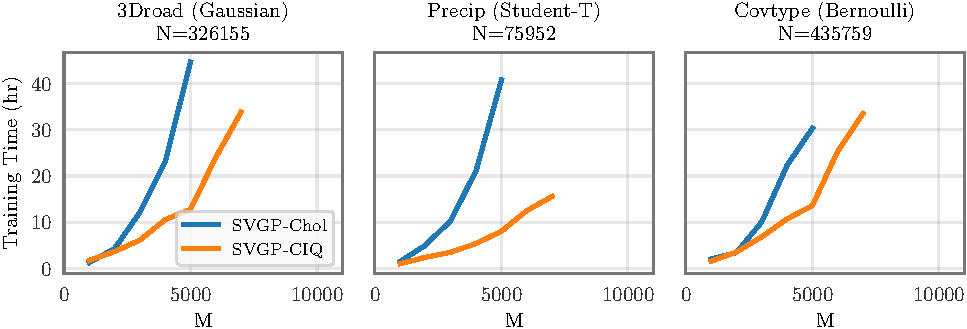
\includegraphics[width=\linewidth]{figures/variational_time.pdf}
  \caption[Train time comparison of Cholesky-whitened vs CIQ-whitened SVGP models.]{
    Train time comparison of Cholesky-whitened vs CIQ-whitened SVGP models.
    {\bf Left:} 3DRoad dataset ($N=326155, D=2$, Gaussian likelihood).
    {\bf Middle:} Precipitation dataset ($N=75952, D=3$, Student-T likelihood).
    {\bf Right:} CoverType dataset ($N=435759, D=54$, Bernoulli likelihood).
    At $M=5,\!000$ inducing points, CIQ is up to $4\times$ faster than Cholesky.
    Moreover CIQ can scale to larger values of $M$ under a fixed computational budget.
  }
  \label{fig:variational_timing}
\end{figure}

\paragraph{Training time.}
In \cref{fig:variational_timing} we plot the training time (in hours) of CIQ/Cholesky models as a function of $M$.
Each model is trained for $20$ epochs on a single NVIDIA Titan-RTX GPU.
Both the Cholesky and CIQ variants take increasingly longer to train as $M$ increases.
Nevertheless, we observe that CIQ models are able to scale to larger $M$ values under a fixed computational budget.
Both CIQ and Cholesky take roughly the same amount of time for $M=1,\!000$ inducing points.
However, CIQ models are roughly $4\times$ faster at $M=5,\!000$.
On the Precipitation dataset, a CIQ model with $M=10,\!000$ finishes training faster than a Cholesky model with $M=5,\!000$.

\begin{figure}[t!]
  \centering
  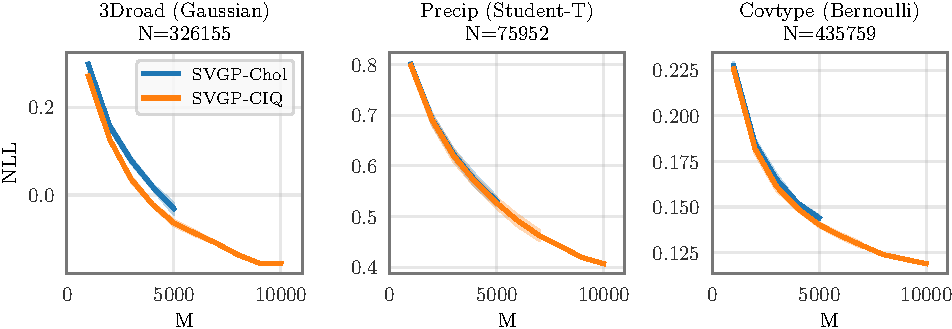
\includegraphics[width=\linewidth]{figures/variational_nll.pdf}
  \caption[Negative log likelihood (NLL) comparison of Cholesky-whitened vs CIQ-whitened SVGP models.]{
    Negative log likelihood (NLL) comparison of Cholesky-whitened vs CIQ-whitened SVGP models.
    {\bf Left:} 3DRoad dataset ($N=326155, D=2$, Gaussian likelihood).
    {\bf Middle:} Precipitation dataset ($N=75952, D=3$, Student-T likelihood).
    {\bf Right:} CoverType dataset ($N=435759, D=54$, Bernoulli likelihood).
    NLL improves with more inducing points ($M$), and Cholesky and CIQ models have similar performance.
    However CIQ scales to larger values of $M$.
  }
  \label{fig:variational_nll}
\end{figure}

\paragraph{Predictive accuracy.}
In exact arithmetic, the CIQ and Cholesky variants of SVGP should produce the exact same computations of $\bK_{\bZ\bZ}^{-1/2} \bb$ up to an orthogonal rotation.
Therefore, we expect that CIQ and Cholesky models with the same number of inducing points should have similar predictive accuracy.
In \cref{fig:variational_nll}, we see that Cholesky and CIQ models achieve do in fact achieve very similar test-set negative log likelihood.
This suggests that the approximations made by the quadrature equation and msMINRES have little impact on performance.

It is worth noting that adaptive gradient optimizers, such as Adam, are not invariant to orthogonal transformation.
Therefore, it is possible that CIQ and Cholesky models may learn slightly different parameters.l
Indeed, we see that on 3droad CIQ models tend to slightly outperform Cholesky models.
Nevertheless, we find that there is not much meaningful predictive difference between these two methods; CIQ however is faster.

Importantly, we find that increasing $M$ does indeed improve the accuracy of models on all datasets.
Scaling from $M=5,\!000$ to $M=10,\!000$ reduced test-set NLL by $0.1$ nats on the 3droad and Precipitation datasets.
We find similar reductions in predictive error (see \cref{app:ngd} for plots).

\begin{figure}[t!]
  \centering
  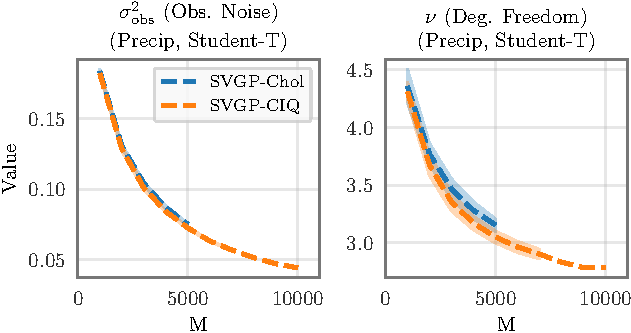
\includegraphics[width=0.7\linewidth]{figures/variational_stats.pdf}
  \caption[Likelihood parameters verses number of inducing points ($M$) for Cholesky-whitened vs CIQ-whitened SVGP models.]{
    Likelihood parameters verses number of inducing points ($M$) for Cholesky-whitened vs CIQ-whitened SVGP models (Precipitation dataset, Student-T likelihood).
    {\bf Left:} observational noise $\sigma^2_\text{obs}$.
    {\bf Right:} degrees of freedom $\nu$.
    As $M$ increases, the estimated obs. noise decreases as does the estimated degrees of freedom (reflecting a heavier-tailed noise distribution).
    This suggests that, with larger $M$, SVGP models can find more signal in the data.
  }
  \label{fig:variational_stats}
\end{figure}

\paragraph{Learned hyperparameters.}
Interestingly, we also find that the learned kernel/likelihood hyperparameters tend to vary significantly with $M$.
For the Precipitation SVGP models, we plot the learned hyperparameters of the Student-T likelihood (see \cref{fig:variational_stats}).
The Student-T likelihood has two learned parameters:
%
\begin{enumerate*}
  \item $\sigma^2_\text{obs}$---which roughly corresponds to variance explained away as observational noise; and
  \item $\nu$ (degrees of freedom)---which controls the tails of the noise model (lower $\nu$ corresponds to heavier tails).
\end{enumerate*}
%
As $M$ increases, we find that the observational noise parameter decreases by a factor of $4$---down from $0.19$ to $0.05$---while the $\nu$ parameter also decreases.
Models with larger $M$ values can more closely approximate the true posterior \cite{hensman2013gaussian}; therefore, we expect that the parameters from the larger-$M$ likelihoods more closely correspond to the true dataset noise.
This confirms findings from \citet{bauer2016understanding}, who argue that variational approximations can tend to overestimate the amount of noise in datasets.
